\documentclass{report}

\usepackage{amsmath}
\usepackage{bookmark}
\usepackage{float}
\usepackage{geometry}
\geometry{
        paper=a4paper,
        top=2cm,
        bottom=2cm,
        left=1.5cm,
        right=1.5cm,
        headheight=0.75cm,
        footskip=1.5cm,
        headsep=0.75cm,
}
\usepackage{hyperref}
\usepackage{mdframed}
\usepackage[normalem]{ulem}
\usepackage{parskip}
\usepackage{tikz}
\usepackage{unicode-math}

\title{Machine Learning Notes}


\begin{document}

\vspace*{2cm}
\begin{center}
	\Huge\textbf{Machine Learning Notes}\\
	\LARGE\textit{an introduction to machine learning}
\end{center}
\vspace*{2cm}

\textit{Machine Learning Notes} \url{https://github.com/cmitsakis/machine-learning-notes} \\
Copyright © 2024 by \textit{Charalampos Mitsakis} \url{https://github.com/cmitsakis} \\
is licensed under \textit{Creative Commons Attribution-ShareAlike 4.0 International (CC-BY-SA 4.0)}. \\
To view a copy of this license, visit \url{https://creativecommons.org/licenses/by-sa/4.0/}


\chapter{Probability Theory}

\section*{Conditional probability}
\[P(A \mid B) = \frac{P(A \cap B)}{P(B)}\]

\section*{Sum rule}
\[P(A)=\sum_n P(A \cap B_n)\]
or, alternatively
\[P(A)=\sum_n P(A \mid B_n) P(B_n)\]

\section*{Product rule}
\[P(A, B) = P(A) P(B \mid A)\]

\section*{Bayes theorem}
\[P(A \mid B) = \frac{P(B \mid A) P(A)}{P(B)}\]
\[P(A_i \mid B) = \frac{P(B \mid A_i) P(A_i)}{\sum\limits_j P(B \mid A_j) P(A_j)}\]

\section*{Probability densities}
\[P[x \in (a, b)] = \int_a^b p(x)\ dx\]
cumulative distribution function:
\[P(z) = \int_{-\infty}^z p(x)\ dx\]
sum rule:
\[p(x) = \int p(x, y)\ dx\]
product rule:
\[p(x, y) = p(x) p(y \mid x)\]

\section*{Expectation}
\[\mathbb{E}[X] := \sum_{i=1}^\infty x_i p_i\]
\[\mathbb{E}[g(X)] := \sum_{x} g(x) p(x)\]
\[\mathbb{E}[X] := \int_{-\infty}^\infty x f(x)\ dx\]
\[\mathbb{E}[g(X)] := \int_{-\infty}^\infty g(x) f(x)\ dx\]
\[\mathbb{E}_{x, y}\left[g(x, y)\right] = \mathbb{E}_x\left[\mathbb{E}_{y|x}[g(x, y)]\right]\]

\section*{Variance and covariance}
\[\begin{split}
	\sigma_x^2 = \operatorname{Var}(X) &:= \mathbb{E}[(X - \mathbb{E}[X])^2] \\
	&= \mathbb{E}[X^2] - \mathbb{E}[X]^2 \\
	&= \operatorname{Cov}(X, X)
\end{split}\]
\[\begin{split}
	\operatorname{cov}(X, Y) &:= E{\left[(X - \mathbb{E}[X])(Y - \mathbb{E}[Y])\right]} \\
	&= \mathbb{E}[X Y] - \mathbb{E}[X] \mathbb{E}[Y]
\end{split}\]
\[r_{xy} := \mathbb{E}[X Y]\]
\[\Sigma_{\symbf{x}} = Cov(\symbf{x}) := \mathbb{E}\left[(\symbf{x} - \mathbb{E}[\symbf{x}])(\symbf{x} - \mathbb{E}[\symbf{x}])^T\right]\]
\[R_{\symbf{x}} := \mathbb{E}[\symbf{x} \symbf{x}^T]\]

\section*{Gaussian Distribution}
$x \sim N(\mu, \sigma^2)$:
\[p(x) = \frac{1}{\sqrt{2 \pi} \sigma} \exp\left(-\frac{(x-\mu)^2}{2\sigma^2}\right)\]

CDF of the standard normal distribution:
\[\Phi(x) = \frac{1}{\sqrt{2\pi}} \int_{-\infty}^x e^{-t^2/2} \, dt\]
\[Q(x) = 1 - Q(-x) = 1 - \Phi(x) = \Phi(-x)\]

$D$-dimensional Gaussian, $\symbf{x} \sim N(\symbf{\mu}, \symbf{\Sigma})$:
\[p(\symbf{x}) = \frac{1}{(2 \pi)^{D/2} |\symbf{\Sigma}|^{1/2}} \exp\left(-\frac{1}{2}(\symbf{x}-\symbf{\mu})^T \symbf{\Sigma}^{-1} (\symbf{x}-\symbf{\mu}) \right)\]

\section*{Entropy}
\[H[X] = - \sum_x p(x) \log_2 p(x)\]


\chapter{Bayesian Decision Theory}

\[P(\omega_i \mid x) = \frac{P(x \mid \omega_i) P(\omega_i)}{P(x)} = \frac{P(x \mid \omega_i) P(\omega_i)}{\sum\limits_j P(x \mid \omega_j) P(\omega_j)}\]

\begin{mdframed}
	\textbf{videos}

	\href{https://www.youtube.com/watch?v=HZGCoVF3YvM}{Bayes theorem, the geometry of changing beliefs [3Blue1Brown]}

	\href{https://www.youtube.com/watch?v=4JscUHGWaB4}{Machine Learning: Bayes Decision Theory}
\end{mdframed}

\section{Minimum Error Classifier (MAP)}
A Bayesian classifier that minimizes the classification error probability.

For two classes:
\[P(\omega_1 \mid x) > P(\omega_2 \mid x) \Rightarrow x \in \omega_1\]
\[P(\omega_2 \mid x) > P(\omega_1 \mid x) \Rightarrow x \in \omega_2\]

equivalently:
\[P(x \mid \omega_1)P(\omega_1) > P(x \mid \omega_2)P(\omega_2) \Rightarrow x \in \omega_1\]
\[P(x \mid \omega_2)P(\omega_2) > P(x \mid \omega_1)P(\omega_1) \Rightarrow x \in \omega_2\]

For many classes:
\[P(\omega_i \mid x) > P(\omega_j \mid x),\ \forall j\ j \neq i \Rightarrow x \in \omega_i\]

Error for two classes. Let $R_1$, $R_2$ be the regions where we decide $\omega_1$ and $\omega_2$ respectively.
\[\begin{split}
	P_e &= P(\symbf{x} \in R_1, \symbf{x} \in \omega_2) + P(\symbf{x} \in R_2, \symbf{x} \in \omega_1) \\
	&= P(\omega_2) \int_{R_1} p(\symbf{x}|\omega_2) \, d\symbf{x} + P(\omega_1) \int_{R_2} p(\symbf{x}|\omega_1) \, d\symbf{x}
\end{split}\]

\section{Minimimum Risk Classifier}
A Bayesian classifier that minimizes the total expected risk. It is useful for cases where some decisions are more important than others.

\subsection*{for two classes:}
\[L = \begin{bmatrix}
	\lambda_{11} & \lambda_{12} \\
	\lambda_{21} & \lambda_{22}
\end{bmatrix}\]
usually:
\[L = \begin{bmatrix}
	0 & \lambda_{12} \\
	\lambda_{21} & 0
\end{bmatrix}\]

\[l_1 = \lambda_{11} p(x \mid \omega_1)P(\omega_1) + \lambda_{21} p(x \mid \omega_2)P(\omega_2)\]
\[l_2 = \lambda_{12} p(x \mid \omega_1)P(\omega_1) + \lambda_{22} p(x \mid \omega_2)P(\omega_2)\]

\[x \in \omega_1 \text{ if } l_1 < l_2 \Leftrightarrow (\lambda_{21}-\lambda_{22}) p(x \mid \omega_2)P(\omega_2) < (\lambda_{12}-\lambda_{11}) p(x \mid \omega_1)P(\omega_1)\]

\[x \in \omega_1 (\omega_2) \text{ if } \frac{p(x \mid \omega_1)}{p(x \mid \omega_2)} > (<) \frac{P(\omega_2)}{P(\omega_1)}\frac{\lambda_{21}-\lambda_{22}}{\lambda_{12}-\lambda_{11}}\]

\section{Discriminant functions}
$g_i (\symbf{x}) \equiv f(P(\omega_i \mid \symbf{x}))$ where $f$ is a monotonically increasing function.

\[g_i(\symbf{x}) > g_j(\symbf{x}),\ \forall j\ j \neq i \Rightarrow x \in \omega_i\]

decision surfaces:
\[g_{ij}(\symbf{x}) \equiv g_i(\symbf{x}) - g_j(\symbf{x}) = 0,\ \forall i, j\ i \neq j\]

\subsection*{Bayesian classification for normal distributions}

\[g_i(\symbf{x}) := \ln (p(\symbf{x} \mid \omega_i) P(\omega_i)) = \ln p(\symbf{x} \mid \omega_i) + \ln P(\omega_i)\]

% Duda's book chapter 2.6 equation (47)
\[g_i(\symbf{x}) = -\frac{1}{2} (\symbf{x} - \symbf{\mu_i})^t \symbf{\Sigma_i}^{-1} (\symbf{x} - \symbf{\mu_i}) - \frac{d}{2}\ln2\pi - \frac{1}{2} ln |\symbf{\Sigma_i}| + ln P(\omega_i)\]

Decision boundary for two classes:
% Theodoridis, 2020, p.309
\[g(\symbf{x}) = g_1(\symbf{x}) - g_2(\symbf{x}) = 0\]
\[\begin{split}
	&\underbrace{\frac{1}{2} \left( \symbf{x}^T \Sigma_2^{-1} \symbf{x} - \symbf{x}^T \Sigma_1^{-1} \symbf{x} \right)}_{\text{quadratic}} \\
	&\underbrace{+ \symbf{\mu}_1^T \Sigma_1^{-1} \symbf{x} - \symbf{\mu}_2^T \Sigma_2^{-1} \symbf{x}}_{\text{linear}} \\
	&\underbrace{- \frac{1}{2} \symbf{\mu}_1^T \Sigma_1^{-1} \symbf{\mu}_1 + \frac{1}{2} \symbf{\mu}_2^T \Sigma_2^{-1} \symbf{\mu}_2 + \ln \frac{P(\omega_1)}{P(\omega_2)} + \frac{1}{2} \ln \frac{|\Sigma_2|}{|\Sigma_1|}}_{\text{constant}} = 0
\end{split}\]

\subsubsection*{Case 1: $\symbf{\Sigma}_i = \sigma^2 \symbf{I}$}
% Duda's book chapter 2.6.1 equation (51)
\[g_i(\symbf{x}) = \symbf{w_i}^t \symbf{x} + w_{i0}\]
where:
\[\symbf{w_i} = \frac{1}{\sigma^{2}} \symbf{\mu_i}\]
\[w_{i0} = -\frac{1}{2\sigma^2}\symbf{\mu_i}^t \symbf{\mu_i} + \ln P(\omega_i) \]

Decision boundary for two classes:
% Theodoridis, 2020, p.310
\[g(\symbf{x}) = (\symbf{\mu_1} - \symbf{\mu_2})^T (\symbf{x} - \symbf{x_0}) = 0\]
it's the perpendicular bisector of the line segment $\symbf{\mu_1} \symbf{\mu_2}$

\subsubsection*{Case 2: $\symbf{\Sigma}_i = \symbf{\Sigma}$}
% Duda's book chapter 2.6.2 equation (58)
\[g_i(\symbf{x}) = -\frac{1}{2} (\symbf{x} - \symbf{\mu_i})^t \symbf{\Sigma_i}^{-1} (\symbf{x} - \symbf{\mu_i}) - \frac{d}{2}\ln2\pi + ln P(\omega_i)\]
\[g_i(\symbf{x}) = \symbf{w_i}^t \symbf{x} + w_{i0}\]
where:
\[\symbf{w_i} = \symbf{\Sigma}^{-1} \symbf{\mu_i}\]
\[w_{i0} = -\frac{1}{2}\symbf{\mu_i}^t \symbf{\Sigma}^{-1} \symbf{\mu_i} + \ln P(\omega_i) \]

Decision boundary for two classes:
% Theodoridis, 2020, p.310
\[g(\symbf{x}) = \symbf{\theta}^T (\symbf{x} - \symbf{x_0}) = 0\]
\[\symbf{\theta} := \symbf{\Sigma}^{-1} (\symbf{\mu_1} - \symbf{\mu_2})\]
\[\symbf{x_0} := \frac{1}{2} (\symbf{\mu_1} + \symbf{\mu_2}) - \ln \frac{P(\omega_1)}{P(\omega_2)} \frac{\symbf{\mu_1} \symbf{\mu_2}}{\left\Vert \symbf{\mu_1} - \symbf{\mu_2} \right\Vert_{\symbf{\Sigma}^{-1}}^2}\]
\[\left\Vert \symbf{\mu_1} - \symbf{\mu_2} \right\Vert_{\symbf{\Sigma}^{-1}} := \sqrt{(\symbf{\mu_1} - \symbf{\mu_2})^T \symbf{\Sigma}^{-1} (\symbf{\mu_1} - \symbf{\mu_2})}\]

\subsubsection*{Case 3: arbitrary $\symbf{\Sigma}_i$}
% Duda's book chapter 2.6.3 equation (64)
\[g_i(\symbf{x}) = \symbf{x}^t \symbf{W_i} \symbf{x} + \symbf{w_i}^t \symbf{x} + w_{i0}\]
where:
\[\symbf{W_i} = -\frac{1}{2}\symbf{\Sigma_i}^{-1}\]
\[\symbf{w_i} = \symbf{\Sigma_i}^{-1} \symbf{\mu_i}\]
\[w_{i0} = -\frac{1}{2}\symbf{\mu_i}^t \symbf{\Sigma_i}^{-1} \symbf{\mu_i} - \ln |\symbf{\Sigma_i}| + \ln P(\omega_i) \]

\subsubsection*{Minimum Eucledian distance classifier}
\begin{itemize}
	\item equiprobable classes
	\item Gaussian distributed with $\symbf{\Sigma}_i = \sigma^2 \symbf{I}$
\end{itemize}

\subsubsection*{Minimum Mahalanobis distance classifier}
\begin{itemize}
	\item equiprobable classes
	\item Gaussian distributed with $\symbf{\Sigma}_i = \symbf{\Sigma}$
\end{itemize}


\chapter{Parameter Estimation}

\section{Maximum Likelihood Estimation}
\begin{mdframed}
	\textbf{videos}

	\href{https://www.youtube.com/watch?v=sguol03tfWo&list=PL5yR0euE9N2kGEf7gqysMFq0Spoq0evNf&index=2}{Machine Learning: Maximum Likelihood Estimation}

	\href{https://www.youtube.com/watch?v=XepXtl9YKwc}{Maximum Likelihood, clearly explained!!!}
\end{mdframed}

We have i.i.d. (independent and identically distributed) random samples $\symbf{X} = [\symbf{x}_1, \ldots, \symbf{x}_n]$ drawn from $p(\symbf{x} \mid \symbf{\theta})$ that follows a distribution that can described by a parameter vector $\symbf{\theta}$.
Find $\symbf{\theta}$ that makes the observed samples the most likely (which means it maximizes $p(\symbf{X} \mid \symbf{\theta})$).

\[\mathcal{L}(\symbf{\theta}) := p(X \mid \symbf{\theta}) = \prod_{k=1}^{n} p(\symbf{x}_k \mid \symbf{\theta})\]

\[\ell(\symbf{\theta}) := \ln \mathcal{L}(\symbf{\theta}) = \sum_{k=1}^n \ln p(\symbf{x}_k \mid \symbf{\theta})\]

\[\begin{split}
	\symbf{\hat \theta}_{\text{ML}} &= \arg\max_{\symbf{\theta}} \mathcal{L}(\symbf{\theta}) \\
	&= \arg\max_{\symbf{\theta}} \ell(\symbf{\theta})
\end{split}\]

Necessary condition for $\symbf{\hat \theta_{\text{ML}}}$:
\[\left. \frac{\partial \mathcal{L}(\symbf{\theta})}{\partial \symbf{\theta}} \right|_{\symbf{\theta} = \symbf{\hat \theta}_{\text{ML}}} = 0\]
or:
\[\begin{split}
	\left. \frac{\partial \ell(\symbf{\theta})}{\partial \symbf{\theta}} \right|_{\symbf{\theta} = \symbf{\hat \theta}_{\text{ML}}} &= \sum_{k=1}^n \frac{\partial \ln p(\symbf{x}_k \mid \symbf{\theta})}{\partial \symbf{\theta}} \\
	&= \sum_{k=1}^n \left( \frac{1}{p(\symbf{x}_k \mid \symbf{\theta})} \frac{\partial p(\symbf{x}_k \mid \symbf{\theta})}{\partial \symbf{\theta}} \right) \\
	&= 0
\end{split}\]

\section{Maximum A Posteriori Probability Estimation}

\[\begin{split}
	\symbf{\hat \theta}_{\text{MAP}} &= \arg\max_{\symbf{\theta}} p(\symbf{\theta} \mid X) \\
	&= \arg\max_{\symbf{\theta}} p(X \mid \symbf{\theta}) p(\symbf{\theta}) \\
	&= \arg\max_{\symbf{\theta}} \ln p(X \mid \symbf{\theta}) + \ln p(\symbf{\theta}) \\
	&= \arg\max_{\symbf{\theta}} \sum_{k=1}^n \left( \ln p(\symbf{x_k} \mid \symbf{\theta}) + \ln p(\symbf{\theta}) \right)
\end{split}\]


\chapter{Linear Regression}

Training data set: $(\symbf{x_n}, \symbf{y_n}),\ n=1, 2, \ldots, N$.

Regression model ($\eta$: noise):
\[y = w_0 + \symbf{w}^T \symbf{x} + \eta = [\symbf{w}^T w_0] \begin{bmatrix}\symbf{x} \\
1\end{bmatrix} + \eta = \symbf{\theta}^T \symbf{x} + \eta\]

Prediction model:
\[\symbf{\hat y} = \symbf{\hat \theta}^T \symbf{x}\]

Cost function:
\[J(\symbf{\theta}) = \sum_{n=1}^N (y_n - \symbf{\theta}^T \symbf{x_n})^2 \]

Estimate $\symbf{\hat \theta}$:
\[\left( \sum_{n=1}^N \symbf{x_n}\symbf{x_n}^T \right) \symbf{\hat \theta} = \sum_{n=1}^N \symbf{x_n} y_n\]
\[\symbf{\hat \theta} = (X^T X)^{-1} X^T \symbf{y}\]

Jointly distributed random variables $\symbf{x}$, $\symbf{y}$:
\[\symbf{\hat y} \equiv \arg\min_{\symbf{\hat y}} E\left[ \left\Vert \symbf{y} - \symbf{\hat y} \right\Vert^2 \right] \equiv \symbf{\hat g}(\symbf{x}) = \mathbb{E}[\symbf{y} | \symbf{x}]\]


\chapter{Neural Networks}

\section*{The Perceptron}

\subsection*{The Perceptron Algorithm}

Training samples: $(y_n, \symbf{x_n}),\ n=1, 2, \ldots, N\ y \in \{-1, +1\}$.

\[\exists \symbf{\theta}_*: \symbf{\theta}_*^T \symbf{x} > 0,\text{ if }\symbf{x} \in \omega_1\text{ and }\symbf{\theta}_*^T \symbf{x} < 0,\text{ if }\symbf{x} \in \omega_2\]

Let $M_{\symbf{\theta}}$ be the set of the samples misclassified by $\symbf{\theta}$.

\[J(\symbf{\theta}) = - \sum_{n: \symbf{x_n} \in M_{\symbf{\theta}}} y_n \symbf{\theta}^T \symbf{x_n}\]

\[y_n = \begin{cases}
	+1, & \text{if } \symbf{x} \in \omega_1 \\
	-1, & \text{if } \symbf{x} \in \omega_2
\end{cases}\]

The perceptron rule:
\[\symbf{\theta}^{(i)} = \symbf{\theta}^{(i-1)} + \mu_i \sum_{n: \symbf{x_n} \in M_{\symbf{\theta}^{(i-1)}}} y_n \symbf{x_n}\]

Pattern-by-pattern version (reward and punishment):
\[\symbf{\theta}^{(i)} = \begin{cases}
	\symbf{\theta}^{(i-1)} + \mu_i y_i \symbf{x}_i, &\text{if } \symbf{x}_i \in M_{\symbf{\theta}^{(i-1)}} \\
	\symbf{\theta}^{(i-1)}, &\text{otherwise}
\end{cases}\]

Neuron:
\[z = \symbf{\theta}^T \symbf{x}\]
\[f(z) = \begin{cases}
	1, & \text{if } z > 0 \\
	0, & \text{if } z < 0
\end{cases}\]

\subsection*{Multilayer Perceptron}

\section*{The Backpropagation Algorithm}

\begin{mdframed}
	\textbf{Study Material}

	\href{http://neuralnetworksanddeeplearning.com/chap2.html}{CHAPTER 2 - How the backpropagation algorithm works}

	\href{https://www.youtube.com/watch?v=Ilg3gGewQ5U&list=PLZHQObOWTQDNU6R1\_67000Dx\_ZCJB-3pi&index=3}{[video] What is backpropagation really doing? | Chapter 3, Deep learning}

	\href{https://www.youtube.com/watch?v=tIeHLnjs5U8&list=PLZHQObOWTQDNU6R1\_67000Dx\_ZCJB-3pi&index=4}{[video] Backpropagation calculus | Chapter 4, Deep learning}

	\href{https://www.youtube.com/watch?v=dB-u77Y5a6A}{[video] Lecture 6: Backpropagation}

	\href{https://www.youtube.com/watch?v=sIX\_9n-1UbM}{[video] Backpropagation Algorithm | Neural Networks}

	\href{https://www.cs.toronto.edu/~rgrosse/courses/csc2541\_2022/tutorials/tut01.pdf}{Tutorial 1 - Backpropagation \& Automatic Differentiation [University of Toronto]}

	\href{https://www.youtube.com/watch?v=VCT1N0EsGj0&list=PLLssT5z\_DsK\_gyrQ\_biidwvPYCRNGI3iv&index=14}{Lecture 3.4 — The backpropagation algorithm — [ Deep Learning | Geoffrey Hinton | UofT ]}
\end{mdframed}

$L$ layers.
$r$-th layer has $k_r$ neurons.
$k_0$ input nodes.

Training samples: $(\symbf{x_n}, \symbf{y_n}),\ n=1, 2, \ldots, N$.

$N$ input vectors:
\[\symbf{x_n} = [x_{n 1}, x_{n 1}, \ldots , x_{n k_0}]^T \in \mathbb{R}^{k_0},\ n = 1, 2, \ldots, N\]

$N$ target output vectors:
\[\symbf{y_n} = [y_{n 1}, y_{n 2}, \ldots , y_{n k_L}]^T \in \mathbb{R}^{k_L},\ n = 1, 2, \ldots, N\]

Output vectors: $\hat y_n$

Let $\symbf{\theta_j^r}$ be the weight vector (including bias) of the $j$th neuron of the $r$th layer:
\[\symbf{\theta_j^r} = [\theta_{j0}^r, \theta_{j1}^r, \ldots, \theta_{jk_{r-1}}^r]^T\]
$\theta_{ji}^r$ denotes the weight from the $i$th neuron of the $(r-1)$th layer to the $j$th neuron of the $r$th layer.

\[\symbf{y_n^r} \equiv [1, y_{n 1}^r, y_{n 2}^r, \ldots, y_{n k_L}^r]^T\]

Iterative step of gradient descent:

\[\symbf{\theta_j^r}(\text{new}) = \symbf{\theta_j^r}(\text{old}) - \mu \left.\frac{\partial J}{\partial \symbf{\theta_j^r}} \right|_{\symbf{\theta_j^r}(\text{old})}\]

\subsection*{The Backpropagation Algorithm}

\begin{mdframed}
\begin{itemize}
	\item Forward pass: compute $y_{nj}^r \forall n, j, r$, using $\symbf{x}_n$ and $\symbf{\theta}_j^r$ 
	\item Backward pass:
	\begin{itemize}
		\item compute $\frac{\partial J}{\partial \symbf{\theta}_j^L},\ j=1, 2, \ldots, k_L$ (last layer)
		\item For $r = L-1 \text{ to } 1$:
		\begin{itemize}
			\item compute $\frac{\partial J}{\partial \symbf{\theta}_k^r},\ k=1, 2, \ldots, k_r$, using the results of the previous layer: $\frac{\partial J}{\partial \symbf{\theta}_j^{r+1}},\ j=1, 2, \ldots, k_{r+1}$
		\end{itemize}
	\end{itemize}
\end{itemize}
\end{mdframed}

For the $k$-th neuron of layer $r$ we have:
\[\symbf{y}_k^r = f\left((\symbf{\theta}_k^r)^T \symbf{y}^{r-1}\right),\ k=1, 2, \ldots, k_r\]

in layer $r$ we have:
\begin{figure}[H]
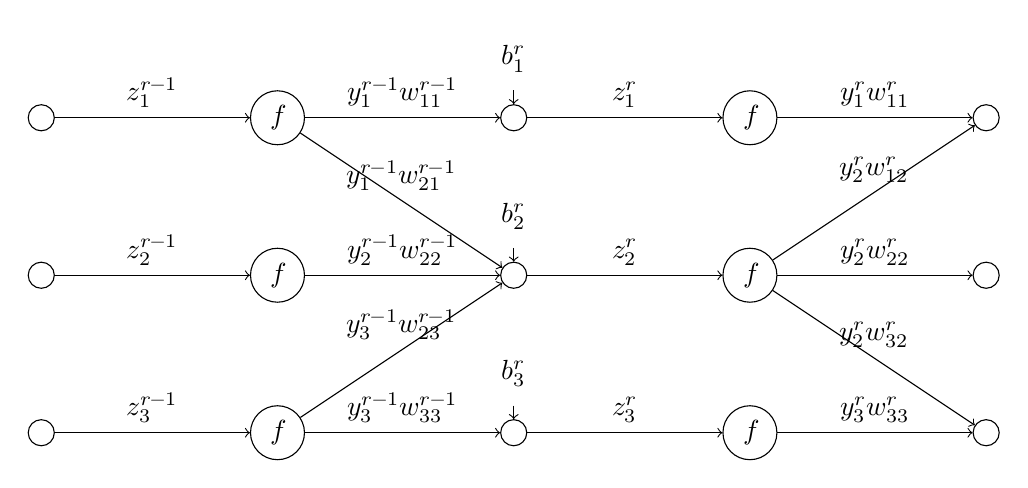
\begin{tikzpicture}
	\node[shape=circle, draw=black] (N11) at (-3, 0) {};
	\node[shape=circle, draw=black] (N21) at (-3, -2) {};
	\node[shape=circle, draw=black] (N31) at (-3, -4) {};

	\node[shape=circle, draw=black] (f11) at (0, 0) {$f$};
	\node[shape=circle, draw=black] (f21) at (0, -2) {$f$};
	\node[shape=circle, draw=black] (f31) at (0, -4) {$f$};

	\node[shape=circle, draw=black] (N12) at (3, 0) {};
	\node[shape=circle, draw=black] (N22) at (3, -2) {};
	\node[shape=circle, draw=black] (N32) at (3, -4) {};

	\node[shape=circle, draw=black] (f12) at (6, 0) {$f$};
	\node[shape=circle, draw=black] (f22) at (6, -2) {$f$};
	\node[shape=circle, draw=black] (f32) at (6, -4) {$f$};

	\node[shape=circle, draw=black] (N13) at (9, 0) {};
	\node[shape=circle, draw=black] (N23) at (9, -2) {};
	\node[shape=circle, draw=black] (N33) at (9, -4) {};

	%\node[shape=circle, draw=black] (f13) at (12, 0) {$f$};
	%\node[shape=circle, draw=black] (f23) at (12, 2) {$f$};
	%\node[shape=circle, draw=black] (f33) at (12, 4) {$f$};

	\node[shape=circle, draw=none] (b12) at (3, 0.75) {$b_1^r$};
	\node[shape=circle, draw=none] (b22) at (3, -1.25) {$b_2^r$};
	\node[shape=circle, draw=none] (b32) at (3, -3.25) {$b_3^r$};

	\path [->] (N11) edge node[above] {$z_1^{r-1}$} (f11);
	\path [->] (N21) edge node[above] {$z_2^{r-1}$} (f21);
	\path [->] (N31) edge node[above] {$z_3^{r-1}$} (f31);

	\path [->] (f11) edge node[above] {$y_{1}^{r-1} w_{11}^{r-1}$} (N12);
	\path [->] (f21) edge node[above] {$y_{2}^{r-1} w_{22}^{r-1}$} (N22);
	\path [->] (f31) edge node[above] {$y_{3}^{r-1} w_{33}^{r-1}$} (N32);
	\path [->] (f11) edge node[above] {$y_{1}^{r-1} w_{21}^{r-1}$} (N22);
	\path [->] (f31) edge node[above] {$y_{3}^{r-1} w_{23}^{r-1}$} (N22);

	\path [->] (N12) edge node[above] {$z_1^r$} (f12);
	\path [->] (N22) edge node[above] {$z_2^r$} (f22);
	\path [->] (N32) edge node[above] {$z_3^r$} (f32);

	\path [->] (f12) edge node[above] {$y_{1}^r w_{11}^r$} (N13);
	\path [->] (f22) edge node[above] {$y_{2}^r w_{22}^r$} (N23);
	\path [->] (f32) edge node[above] {$y_{3}^r w_{33}^r$} (N33);
	\path [->] (f22) edge node[above] {$y_{2}^r w_{12}^r$} (N13);
	\path [->] (f22) edge node[above] {$y_{2}^r w_{32}^r$} (N33);
	
	%\path [->] (N13) edge node[above] {$z_1^{r+1}$} (f13);
	%\path [->] (N23) edge node[above] {$z_2^{r+1}$} (f23);
	%\path [->] (N33) edge node[above] {$z_3^{r+1}$} (f33);

	\path [->] (b12) edge node[above] {} (N12);
	\path [->] (b22) edge node[above] {} (N22);
	\path [->] (b32) edge node[above] {} (N32);

\end{tikzpicture}
\end{figure}

\textbf{Forward pass - calculations for layer r}

\[z_j^r = \sum_{n=1}^{k_{r-1}} \left( w_{in}^r y_n^{r-1} \right) + b_j^r,\ j=1, 2, \ldots, k_r\]
\[y_j^r = f(z_j^r),\ j=1, 2, \ldots, k_r\]

\textbf{Backward pass - calculations for layer L (last)}

\[\overline{z_j^L} = \overline{y_j^L} f'(z_j^L)\]

\textbf{Backward pass - calculations for layer r}

(notation: $\overline{a} \equiv \frac{\partial J}{\partial a}$)

Using $\overline{y^r}$ (we calculated on layer $r+1$), for $j=1, \ldots, k_r$ we calculate the following:

\[\overline{z_j^r} = \overline{y_j^r} f'(z_j^r)\]

\[\overline{y_j^{r-1}} = \sum_{n=1}^{k_{r}} \frac{\partial z_n^r}{\partial y_j^{r-1}} \overline{z_n^r} = \sum_{n=1}^{k_{r}} w_{jn}^r \overline{z_n^r}\]

\[\overline{w_{ji}^r} = \overline{z_j^r} y_i^{r-1},\ i=1, \ldots, k_{r-1}\]

\[\overline{b_j^r} = \overline{z_j^r}\]

\[\overline{z_j^{r-1}} = \overline{y_j^{r-1}} f'(z_j^{r-1})\]

\textbf{Multivariate Chain Rule}
\[\frac{\partial}{\partial t} f(x(t), y(t)) = \frac{\partial f}{\partial x} \frac{\partial x}{\partial t} + \frac{\partial f}{\partial y} \frac{\partial y}{\partial t}\]
\[\overline{t} = \overline{x} \frac{\partial x}{\partial t} + \overline{y} \frac{\partial y}{\partial t}\]

\textbf{sigmoid function}
\[\sigma(x) = \frac{1}{1+e^{-at}}\]
\[\sigma'(x) = a \sigma(x) (1-\sigma(x))\]

\end{document}
